\documentclass{beamer}
\usepackage{listings}
\lstset{
%language=C,
frame=single, 
breaklines=true,
columns=fullflexible
}
\usepackage{subcaption}
\usepackage{url}

\usepackage{tikz}
\usepackage{pgfplots}
\pgfplotsset{compat=1.17}
\usepackage{tkz-fct}
\usepackage{mathrsfs}
\usepackage{txfonts}
\usepackage{tkz-euclide} 
\usetikzlibrary{calc,math}
\usepackage{float}
\newcommand\norm[1]{\left\lVert#1\right\rVert}
\renewcommand{\vec}[1]{\mathbf{#1}}
\providecommand{\pr}[1]{\ensuremath{\Pr\left(#1\right)}}
\usepackage[export]{adjustbox}
\usepackage[utf8]{inputenc}
\usepackage{amsmath}
\usetheme{Boadilla}
\title{CSIR UGC NET EXAM (June 2016), Q.118}
\author{Tanmay Garg - EE20BTECH11048}

\begin{document}
\begin{frame}
\titlepage
\end{frame}
\section{Question}
\begin{frame}
\frametitle{CSIR UGC NET EXAM (June 2016), Q.118}
\begin{block}{Question}
Three types of components are used in electrical circuits 1, 2, 3 as shown below in the figure
Suppose that each of the three components fail with probability $p$ and independently of each other. Let $q_i = \pr{\text{Circuit $i$ does not fail}}$; $i=1,2,3$ For $0<p<1$, we have
    \begin{enumerate}
        \item $q_3>q_1$
        \item $q_2=q_1$
        \item $q_2>q_1$
        \item $q_2>q_3$
    \end{enumerate}
\end{block}
\end{frame}
\begin{frame}{Question}
\begin{block}{Figure}
\begin{figure}[h]
    \centering
    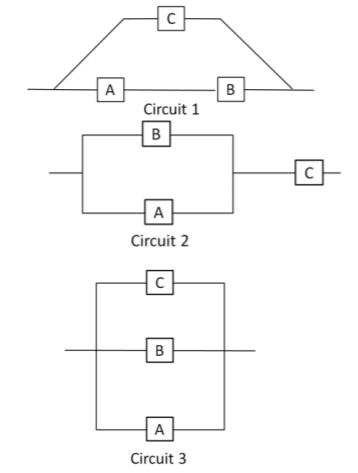
\includegraphics[width=0.3\columnwidth]{circuits.png}
    \caption{Circuits}
    \label{fig:fig_label}
\end{figure}
\end{block}

\end{frame}
\section{Boolean Algebra}
\begin{frame}{Boolean Algebra}
\begin{block}{Boolean Expression for Series Circuit}
     Boolean Expression for series circuit:
     \begin{align}
         AB
     \end{align}
     \begin{figure}
        \centering
        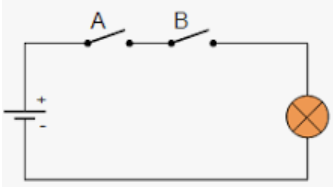
\includegraphics{boolean1.png}
        \caption{Series}
        \label{boolean1}
    \end{figure}
\end{block}
    
\end{frame}
\begin{frame}{Boolean Algebra}
\begin{block}{Boolean Expression for Parallel Circuit}
     Boolean Expression for parallel circuit:
     \begin{align}
         A+B
     \end{align}
     \begin{figure}
        \centering
        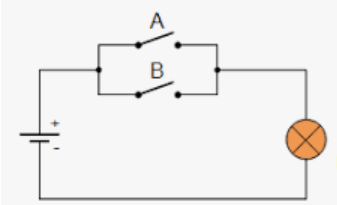
\includegraphics{boolean2.png}
        \caption{Parallel}
        \label{boolean2}
    \end{figure}
\end{block}
    
\end{frame}
\section{Solution}
\subsection{Circuit 1}
\begin{frame}{Circuit 1}
\begin{block}{Boolean Expression}
The Boolean Algebraic expression for this circuit is:
    \begin{figure}
        \centering
        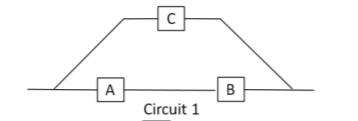
\includegraphics{circuit1.png}
        \caption{Circuit 1}
        \label{cir1_label}
    \end{figure}
    We get:
    \begin{align}
        AB + C
    \end{align}
\end{block}
\end{frame}
\begin{frame}{Circuit 1}
\begin{block}{Probabilities}
    For Circuit 1 to work the truth table will be:
    \begin{table}[h]
    \centering
    \begin{tabular}{|c|c|c|c|c|}
    \hline
         $A$ & $B$ & $C$ & $(AB) + C$& Probability \\
         \hline
         1 &1  & 0 &1 &$p(1-p)^2$\\\hline
         1&1&1&1&$(1-p)^3$\\\hline
         0&1&1&1&$p(1-p)^2$\\\hline
         0&0&1&1&$p^2(1-p)$\\\hline
         1&0&1&1&$p(1-p)^2$\\
    \hline
    \end{tabular}
    \caption{Circuit 1 working}
    \label{table_1}
\end{table}
    Adding all we get $\pr{\text{Circuit 1 works}}$ :
    \begin{align}
        q_1 = p^3-2p^2+1 \label{q_1_label}
    \end{align}
\end{block}
\end{frame}
\subsection{Circuit 2}

\begin{frame}{Circuit 2}
\begin{block}{Boolean Expression}
    The Boolean Algebraic expression for this circuit is:
    \begin{figure}
        \centering
        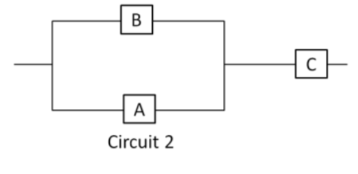
\includegraphics{circuit2.png}
        \caption{Circuit 2}
        \label{cir2_label}
    \end{figure}
    We get:
    \begin{align}
        (A+B)C
    \end{align}
\end{block}
\end{frame}
\begin{frame}{Circuit 2}
\begin{block}{Probabilities}
    For Circuit 2 to work the truth table will be:
    \begin{table}[h]
    \centering
    \begin{tabular}{|c|c|c|c|c|}
    \hline
         $A$ & $B$ & $C$ & $(A+B)C$& Probability\\
         \hline
         1&1&1&1 &$(1-p)^3$\\ \hline
         1&0&1&1& $p(1-p)^2$\\\hline
         0&1&1&1& $p(1-p)^2$\\
    \hline
    \end{tabular}
    \caption{Circuit 2 working}
    \label{tab:table2}
\end{table}
    Adding all we get $\pr{\text{Circuit 2 works}}$:
    \begin{align}
    q_2 = p^3-p^2-p+1 \label{q_2_label}
\end{align}
\end{block}
\end{frame}

\subsection{Circuit 3}

\begin{frame}{Circuit 3}
\begin{block}{Boolean Expression}
    The Boolean Algebraic expression for this circuit is:
    \begin{figure}
        \centering
        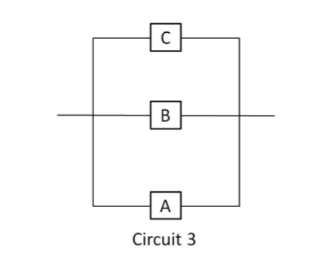
\includegraphics[width=0.3\columnwidth]{circuit3.png}
        \caption{Circuit 3}
        \label{cir2_label}
    \end{figure}
    We get:
    \begin{align}
        A + B + C
    \end{align}
\end{block}
    
\end{frame}
\begin{frame}{Circuit 3}
\begin{block}{Probabilities}
    For Circuit 3 to work the truth table will be:
    \begin{table}[h]
    \centering
    \resizebox{0.45\columnwidth}{!}{
    \begin{tabular}{|c|c|c|c|c|}
    \hline
         $A$ & $B$ & $C$ & $A + B + C$ & Probability \\
         \hline
         1&0&0&1 & $p^2(1-p)$\\\hline
         0&1&0&1& $p^2(1-p)$\\\hline
         0&0&1&1& $p^2(1-p)$\\\hline
         1&1&0&1& $p(1-p)^2$\\\hline
         1&0&1&1& $p(1-p)^2$\\\hline
         0&1&1&1& $p(1-p)^2$\\\hline
         1&1&1&1& $(1-p)^3$\\
    \hline
    \end{tabular}
    }
    \caption{Circuit 3 working}
    \label{tab:table3}
\end{table}
    Adding all we get $\pr{\text{Circuit 3 works}}$:
    \begin{align}
    q_3 = 1-p^3 \label{q_3_label}
\end{align}
\end{block}
\end{frame}


\subsection{Plots}

\begin{frame}{Plotting the functions}
\begin{block}{Graph}
    Plotting \eqref{q_1_label}, \eqref{q_2_label} and \eqref{q_3_label}
    
\begin{center}
    \begin{tikzpicture}
\pgfplotsset{%
    width=0.52\textwidth,
    height=0.5\textwidth
}
\begin{axis}[
    axis lines = left,
    xlabel = $p$,
    ylabel = {$f(p)$},
]
\addplot [
    domain=0:1, 
    samples=100, 
    color=red,
]
{x^3-2*x^2+1};
\addlegendentry{$q_1$}
\addplot [
    domain=0:1, 
    samples=100, 
    color=blue,
    ]
    {x^3-x^2-x+1};
\addlegendentry{$q_2$}
\addplot [
    domain=0:1, 
    samples=100, 
    color=green,
]
{1-x^3};
\addlegendentry{$q_3$}
\end{axis}
\end{tikzpicture}
\end{center}

\end{block}
    
\end{frame}
\subsection{Answer}

\begin{frame}{Answer}
\begin{block}{Correct Answer}
     On comparing from the graph we can determine that:
    \begin{align}
    \therefore q_3>q_1>q_2
\end{align}
    Hence \textbf{Option 1}: $q_3>q_1$ is correct
\end{block}
   
\end{frame}
\end{document}